\newpage
\section{TGGs in action}
\genHeader
\label{sect:TGGs_in_Action}

Before we can execute our rules, we need to create something for the TGG to transform. In other words, we need to create an instance model\footnote{For a
detailed review how to create instances, refer to Part~II, Section~3} of either our target or our source metamodel! Since dictionaries are
of a much simpler structure, let's start with the backwards transformation.

\begin{itemize}

\item[$\blacktriangleright$] Navigate to \texttt{Dictionary\-Language/model/} and open \texttt{Dictio\-nary\-Lang\-uage.ecore}. Expand the tree and create a new dynamic instance of a \texttt{Dictionary} named \texttt{bwd.src.xmi} (choose the EClass \texttt{Dictionary}, right-click, and select \texttt{Create dynamic instance}). 
Make sure you persist your instance as \texttt{Learn\-ing\-Box\-To\-Dictionary\-In\-te\-gra\-tion/in\-stan\-ces/bwd.src.xmi} (as depicted in \Cref{eclipse:create_instance_dict}).

\begin{figure}[htbp]
\begin{center}
  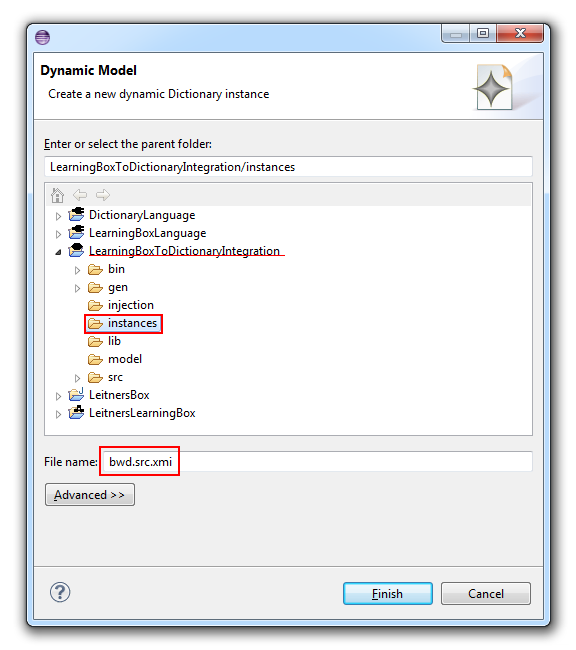
\includegraphics[width=0.8\textwidth]{eclipse_dictionaryInstance}
  \caption{Create a dynamic instance of \texttt{Dictionary}}
  \label{eclipse:create_instance_dict}
\end{center}
\end{figure}

\newpage

\item[$\blacktriangleright$] Open the new file and edit the \texttt{Dictionary} properties by double-clicking and setting \texttt{Title} to \texttt{English Numbers} in the \texttt{Properties} tab below the window.

\vspace{0.5cm}

\item[$\blacktriangleright$] Create three child \texttt{Entry} objects.
Don't forget the syntax we decided upon for each \texttt{entry.content} in the \texttt{CardToEntryRule} when setting up the constraints! 
Be sure to set this property according to the format \texttt{<word>:<meaning>}. 
Give each \texttt{entry} a different difficulty \texttt{level}, e.g., \texttt{beginner} for \texttt{One:Eins}, \texttt{advanced} for \texttt{Two:Zwei}, and \texttt{master} for \texttt{Three:Drei}.
Your instance should resemble \Cref{eclipse:dictionaryxmi}.
After this works you should of course play around with the model and add all kind of cards to see what happens.

\begin{figure}[htbp]
\begin{center}
  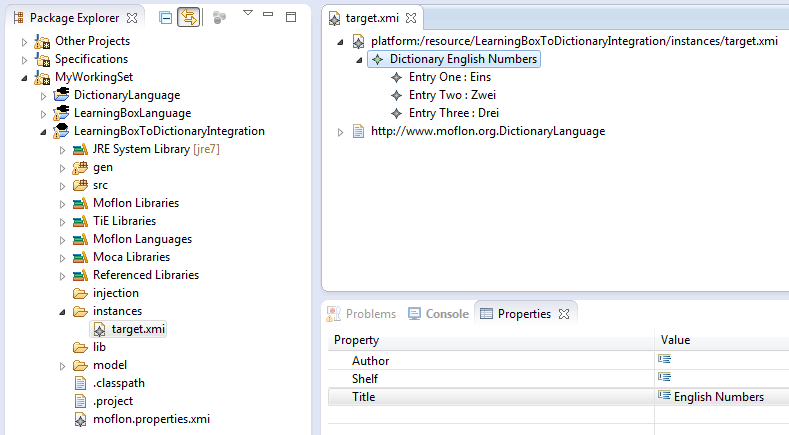
\includegraphics[width=0.9\textwidth]{eclipse_targetThreeEntries}
  \caption{Fill a \texttt{Dictionary} for the transformation}
  \label{eclipse:dictionaryxmi}
\end{center}
\end{figure}

\item[$\blacktriangleright$] eMoflon generates default stubs to execute the transformation.
Navigate to ``LearningBox\-To\-Dictionary\-In\-te\-gra\-tion\-/\-src/\-org.\-mof\-lon.\-tie'' and open \texttt{Learn\-ing\-Box\-To\-Dict\-ion\-ary\-Int\-e\-grat\-ion\-Trafo.\-java}.

\item[$\blacktriangleright$] As you can see, this file is a driver for forward and backward transformations, transforming a source \texttt{box} to a target \texttt{dictionary}, and backward from a \texttt{dictionary} to a \texttt{box}. 
As this is good old Java code, you can adjust everything as you wish.
To follow this handbook, however, do not change anything for the moment.

\item[$\blacktriangleright$] Right-click the file in the Package Explorer and navigate to ``Run as\ldots/Java Application'' to execute the file.

\item[$\blacktriangleright$] Did you get one error message, followed by one success message in the eMoflon console window (\Cref{eclipse:tggERROR}) below
the editor? Perfect! Both of these statements make sense -- our TGG first attempted the forward transformation but, given that it was missing the source
(\texttt{box}) instance, it was only able to perform a transformation in the backwards direction.
The stub checks for \texttt{fwd.src.xmi} and \texttt{bwd.src.xmi} files per convention (all this can of course be edited and changed).

\begin{figure}[htbp]
\begin{center}
  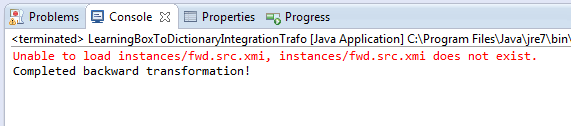
\includegraphics[width=\textwidth]{eclipse_TGGError}
  \caption{Running the backward transformation}
  \label{eclipse:tggERROR}
\end{center}
\end{figure}

\item[$\blacktriangleright$] Refresh the integration project's \texttt{instances} folder. 
Three new \texttt{.xmi} files should have appeared representing your backward triple. 
While you created the \texttt{bwd.src.xmi} instance, the TGG generated \texttt{bwd.corr.xmi}, the correspondence graph between target and source, \texttt{bwd.protocol.xmi}, a directed acyclic graph of the rule applications that lead to this result, and \texttt{bwd.trg.xmi}, the output of the transformation. 

\item[$\blacktriangleright$] If you open and inspect \texttt{bwd.trg.xmi} you'll find that it's a \texttt{Box} of \texttt{English Numbers}.
Expand the tree and you'll see our \texttt{Dictionary} in its corresponding
\texttt{Box} format containing three \texttt{Par\-ti\-tions} (\Cref{eclipse:derivedBOX}). 
Double click each \texttt{card} and observe how each \texttt{entry.content} was successfully split into two sides.
Also note how the cards were placed in the correct (at least according to our \texttt{indexToLevel} attribute condition) partition.

\begin{figure}[htbp]
\begin{center}
  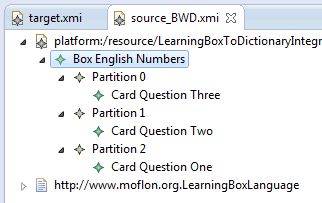
\includegraphics[width=0.5\textwidth]{eclipse_derivedSource}
  \caption{Result of the \emph{backwards} transformation}
  \label{eclipse:derivedBOX}
\end{center}
\end{figure}

\item[$\blacktriangleright$] Congratulations! You have successfully performed your first \emph{backward} transformation using TGGs!
To understand better what happened, eMoflon provides two important tools: the first is the correspondence model containing all established links between source and target elements, the second is the so called protocol of the transformation. 

\item[$\blacktriangleright$] Go ahead and open \texttt{bwd.corr.xmi}.
This model contains the created correspondence model, and references both source and target models.
Using eMoflon's \texttt{Abstract Syntax View}, you can drag in a selection of elements and explore (right-click on a node in the view to choose if direct neighbours or all transitive neighbours should be added to the view) how the models are connected.
You can remove elements from the view, zoom in and out, and also pick from a choice of standard layout algorithms.
\Cref{eclipse:graphView} shows all three complete models in the view with all correspondence links highlighted. 
You can choose elements in the view to see their attribute values either as a tool tip, or in the standard properties view in Eclipse.

\begin{figure}[htb]
\begin{center}
  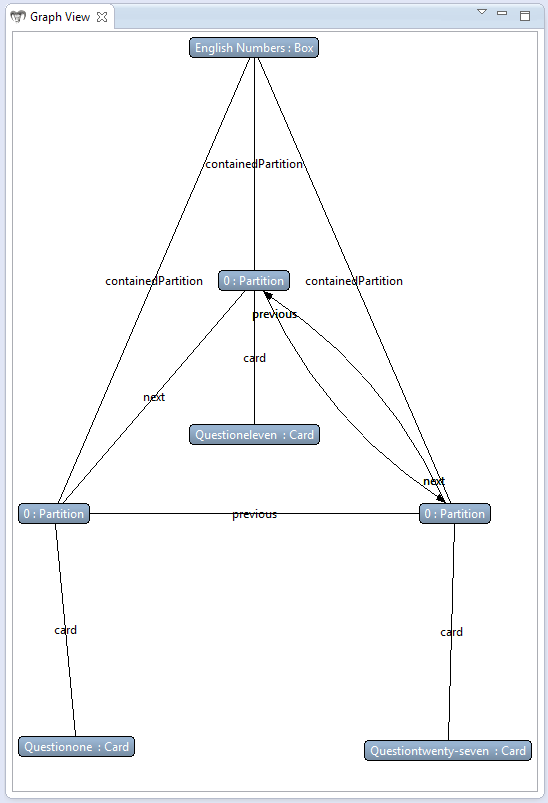
\includegraphics[width=\textwidth]{eclipse_EngNumBoxGraphView}
  \caption{Inspecting the correspondence models}
  \label{eclipse:graphView}
\end{center}
\end{figure}

\item[$\blacktriangleright$] eMoflon provides a special visualisation for protocol models, so go ahead and open \texttt{bwd.protocol.xmi}.
This time around, use the PlantUML view to inspect the protocol.
If you select the root element (\texttt{Precedence Structure}), you'll see a tree of \emph{rule applications}, showing you which rules were applied to achieve the result.
As \texttt{Card\-To\-Entry\-Rule} can only be applied after \texttt{BoxToDictionaryRule}, an application of the latter is a parent for all other rule applications.
These are all children on the same level, as the exact order of application is irrelevant in this case.
This, in general, directed acyclic graph of rule applications is depicted in \Cref{eclipse_protocol}.
 
\begin{figure}[htb]
\begin{center}
  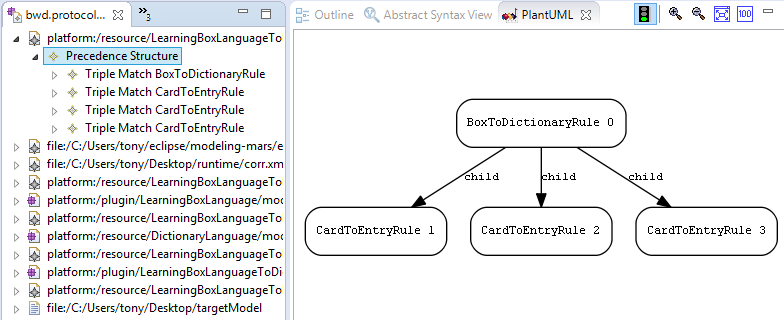
\includegraphics[width=\textwidth]{eclipse_protocol}
  \caption{Inspecting the protocol}
  \label{eclipse_protocol}
\end{center}
\end{figure}

\begin{figure}[htb]
\begin{center}
  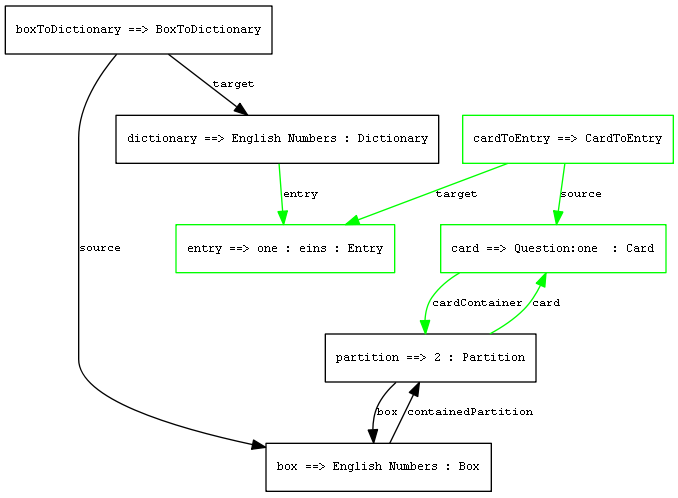
\includegraphics[width=0.9\textwidth]{eclipse_ruleApplication}
  \caption{Inspecting a rule application}
  \label{eclipse_ruleApplication}
\end{center}
\end{figure}

\item[$\blacktriangleright$] To inspect a rule application, choose one of the children of the precedence structure in the tree view.
If you choose, for example, a \texttt{Card\-To\-Entry\-Rule} node, a diagram similar to that depicted in \Cref{eclipse_ruleApplication} will be shown as a visualisation of the rule application.
To understand this diagram, note that the labels of the nodes are of the form \texttt{rule variable ==> model element}, showing how the object and link variables in the rule were ``matched'' to actual elements in the source and target models.
The colours indicate which elements would be created by applying this rule (in the simultaneous evolution of all three models).
This protocol is not only for documentation, but is also used for model synchronisation, which we'll discuss and try out in a moment.

\item[$\blacktriangleright$] To convince yourself that the transformation is actually bidirectional, create a source model, and run the TGG again to perform a \emph{forwards} transformation of a \texttt{Box} into a \texttt{Dictionary}.
The easiest way to do this is to make a copy of \texttt{bwd.trg.xmi} and rename
it to \texttt{fwd.src.xmi}.

\item[$\blacktriangleright$] Run \texttt{LearningBoxToDictionaryIntegrationTrafo} again and refresh the ``instances'' folder. 
Compare the output \texttt{fwd.trg.xmi} against the original \texttt{bwd.src.xmi} Dictionary model. 
If everything went right, they should be isomorphic (identical up to perhaps sorting of children).
\end{itemize}

%%% Local Variables: 
%%% mode: latex
%%% TeX-master: "../src/TGG_mainFile"
%%% End: 
